\subsection{ Zr($10\bar{1}0$) surface.}
\begin{frame}{ Zr($10\bar{1}0$) surface, alloy segregation and Hydrogen Absorption}
  
  This project is carried on in colaboration with Fernando Soto, a Postdoc at 
  Perla Balbuena's group in Texas A\&M University, USA. 

  \begin{block}{Progress so far}
  \begin{itemize}
      \item<1-> Ta and V segregate differently than Nb and Sn
	\begin{center}
	  $\vcenter{ 
	  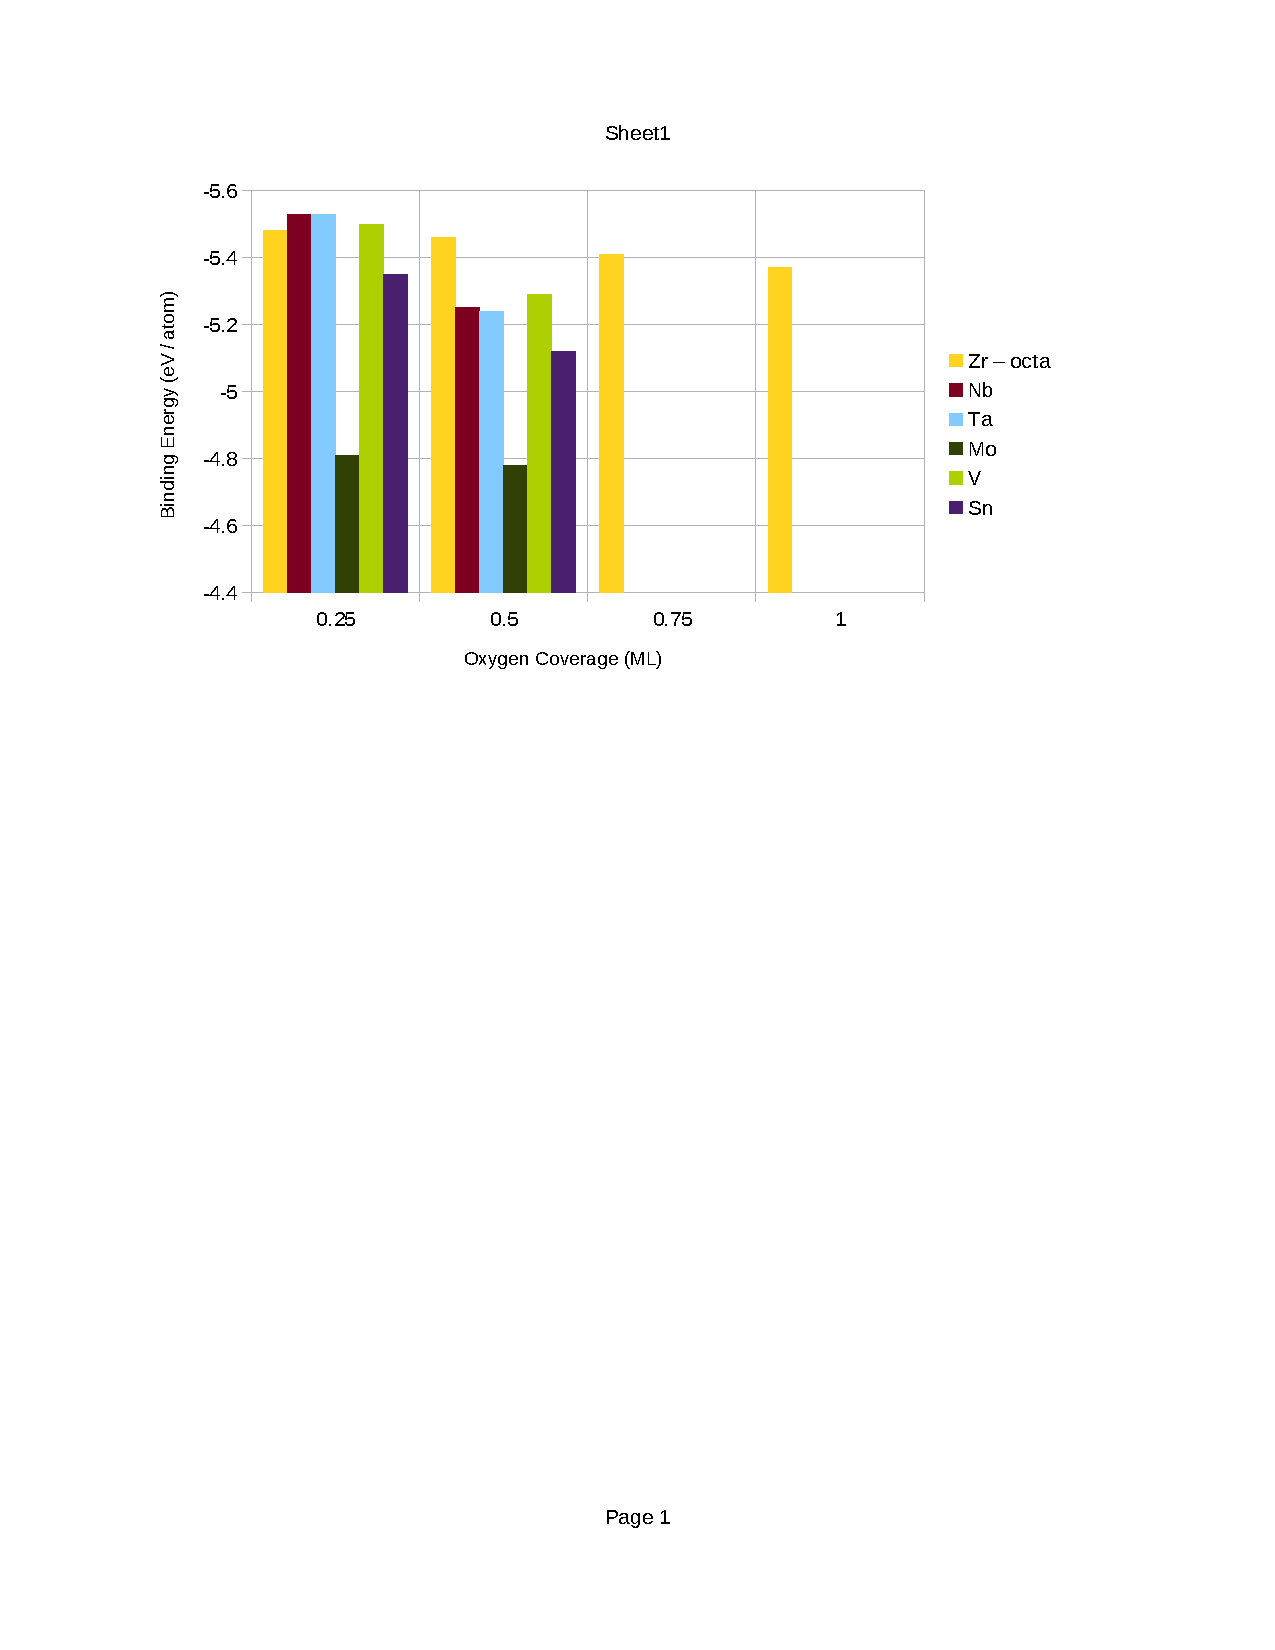
\includegraphics[height=3.5cm,trim={1cm 16.5cm 5cm 3cm},clip]
	  {./02-CurrentResearch/OxygenBindingEnergy.pdf}<1>
	  }$
	\end{center}
      \item<2> Hydgrogen moves differently in the presence of Ta and V,
	\begin{center}
	$\vcenter{
	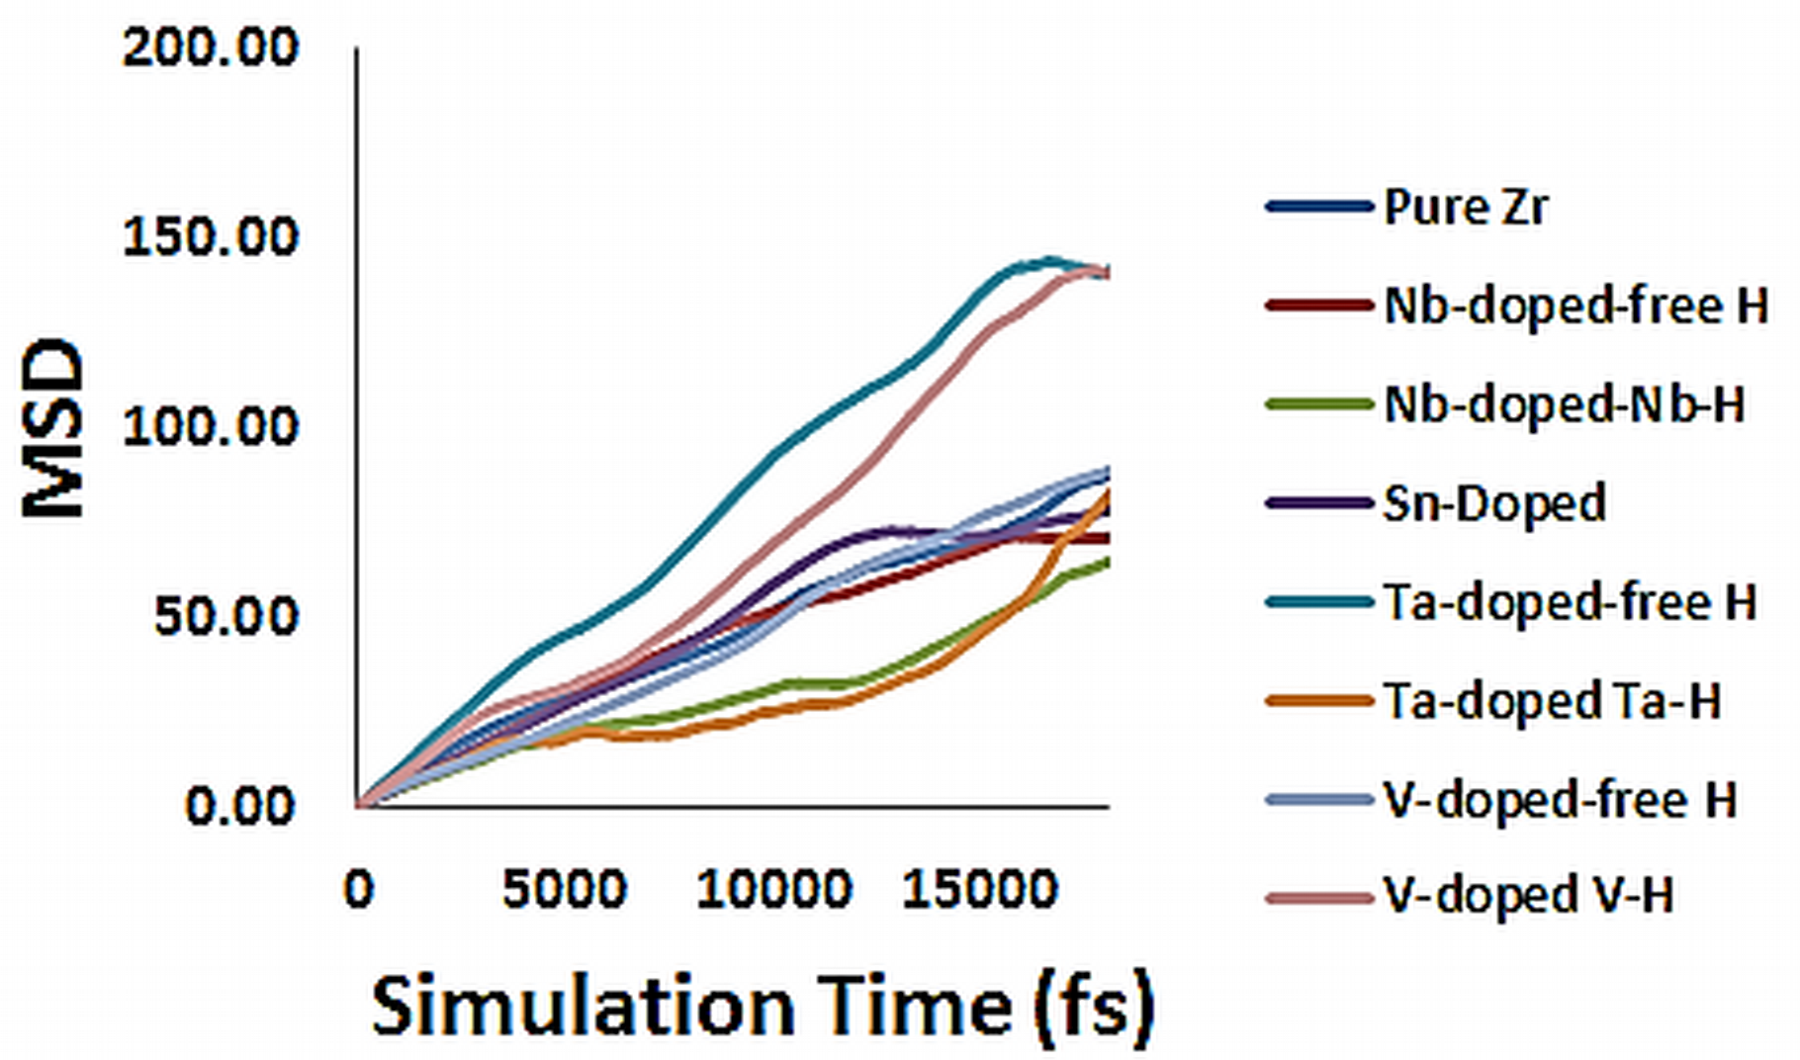
\includegraphics[height=4cm]{./02-CurrentResearch/HydrogenMeanFreePaths.png}
	  }$
	\end{center}
  \end{itemize}
  \end{block}

\end{frame}
